\chapter{RESEARCH METHODOLOGY}

\section{Research Design and Software Engineering Life Cycle}

This research develops an open-source, web-based decision support system designed to automate the ingestion, multi-ratio petrophysical analysis, real-time visualization, and deterministic fluid forecasting of Gas While Drilling (GWD) data. Because the platform delivers an interactive computational tool for operational geoscience, the methodology follows a structured five-stage Software Development Life Cycle (SDLC) adapted for scientific computing:

\begin{enumerate}
    \item \textbf{Requirements Analysis and Specification:} Formulating functional requirements (multi-format mud log parsing, automated 16-parameter ratio computation, deterministic fluid classification, and 21-track depth-registered visualization) and non-functional requirements (sub-5-second processing latency, mathematical auditability, and open-source accessibility). Requirements were established through domain feedback from practicing petrophysicists, operations geologists, and wellsite engineers.
    
    \item \textbf{System and Architectural Design:} Structuring the platform using a decoupled three-tier software architecture comprising a Data Ingestion Layer, a Deterministic Logic Engine Layer, and a Reactive Presentation Layer. The core calculation pipeline models petrophysical dependencies as a declarative directed acyclic graph, supporting dynamic parameter customization and live schema management.
    
    \item \textbf{Software Implementation:} Implementing modular Python packages (\texttt{parser.py}, \texttt{engine.py}, \texttt{evaluator.py}, and \texttt{app.py}) using vectorized numerical routines (NumPy, Pandas) and reactive web components (Dash, Plotly). Because the calculation core operates strictly on closed-form petrophysical formulas and explicit boundary thresholds, the system undergoes a data-free deterministic build phase requiring no stochastic model training.
    
    \item \textbf{System Verification and Multi-Tier Evaluation:} Conducting comprehensive validation spanning algorithmic unit verification against analytical reference values, empirical classification benchmarking against ground-truth well tests using multi-class classification metrics (Accuracy, Precision, Recall, Macro-$F_1$) \citep{sokolova2009, powers2011}, computational latency profiling ($\Delta t_{\text{total}} \le 5.0\text{ s}$), and observational user testing ($S_{\text{user}} > 68.0$).
    
    \item \textbf{Packaging and Open-Source Deployment:} Assembling standardized environment manifests (\texttt{requirements.txt}) and releasing the source code on a public repository to facilitate reproducible formation evaluation and academic research.
\end{enumerate}

\section{Requirements Analysis and Specification}

Establishing structured software specifications ensures that the developed application addresses operational challenges in formation evaluation while maintaining computational efficiency and system reliability.

\subsection{Functional Requirements (FR)}
The functional specifications define the operational capabilities delivered by the system:
\begin{itemize}
    \item \textbf{FR-01 (Multi-Format Ingestion):} Ingest raw mud logging files across standard tabular and delimited text formats (\texttt{.txt}, \texttt{.csv}, \texttt{.xlsx}, and \texttt{.las}), automatically isolating data records from variable company headers.
    \item \textbf{FR-02 (Continuous Data Normalization):} Validate, align, and clean chromatographic gas curves ($C_1$ through $C_5$) against continuous Measured Depth ($MD$) indices, systematically handling missing or non-positive values.
    \item \textbf{FR-03 (Automated Multi-Ratio Computation):} Automatically compute 16 derived petrophysical indicators from input gas curves upon file upload.
    \item \textbf{FR-04 (Deterministic Fluid Zone Forecasting):} Apply closed-form decision-tree logic to classify depth increments into categorical fluid regimes: Gas Zone, Oil Zone, or Water/Non-Productive Sand.
    \item \textbf{FR-05 (Multi-Track Depth-Synchronized Visualization):} Render continuous vertical area charts for all computed indicators and fluid zones across 21 dedicated tracks, featuring synchronized scrolling, depth zooming, and cursor tooltips.
    \item \textbf{FR-06 (Dynamic Schema and Formula Management):} Enable interactive column visibility toggling, track reordering, and live formula and cutoff threshold customization with immediate preview updates.
    \item \textbf{FR-07 (Data Export and Reporting):} Enable the export of computed petrophysical curves and classification summaries in standardized tabular formats.
\end{itemize}

\subsection{Non-Functional Requirements (NFR)}
Non-functional specifications ensure software robustness, responsiveness, and professional auditability:
\begin{itemize}
    \item \textbf{NFR-01 (Computational Latency):} The end-to-end execution pipeline (file ingestion, ratio calculation, and multi-track visual rendering) must complete in under 5.0 seconds for well trajectories exceeding 3,000 meters.
    \item \textbf{NFR-02 (Mathematical Auditability):} All calculations must operate on explicit, transparent formulas with zero non-traceable parameters, ensuring complete compliance with SPE PRMS reserve certification standards \citep{ref3}.
    \item \textbf{NFR-03 (Usability and Workflow Learnability):} The interface must deliver an intuitive single-click operational workflow accessible without specialized software training, targeting a mean usability score of $\overline{S} > 68.0/100$.
    \item \textbf{NFR-04 (Accessibility and Open Distribution):} The application must run on open-source Python technologies, eliminating multi-thousand-dollar annual commercial licensing constraints \citep{wood2020}.
\end{itemize}

\subsection{Requirements Elicitation}
Requirements were synthesized through domain surveys and consultations with practicing wellsite engineers, operations geologists, and petrophysicists. The feedback highlighted operational preferences for instantaneous multi-ratio cross-comparison, customizable threshold cutoffs, and responsive multi-track visual layouts that mirror standardized wellsite strip log templates.

\section{System Architecture and Design}

To ensure separation of concerns, high maintainability, and low computational overhead, the software is structured as a decoupled three-tier architecture.

\subsection{Three-Tier Architectural Overview}
The system architecture separates data processing into three dedicated layers:
\begin{enumerate}
    \item \textbf{Data Parsing \& Ingestion Layer (\texttt{parser.py}):} Handles file decoding, format identification, header stripping, data cleaning, and structured matrix generation.
    \item \textbf{Deterministic Logic Engine Layer (\texttt{engine.py} \& \texttt{evaluator.py}):} Implements petrophysical formulas, maintains the declarative parameter dependency graph, vectorizes numerical operations, and executes zone classification logic.
    \item \textbf{Presentation \& Dashboard Layer (\texttt{app.py}):} Provides an interactive, reactive web user interface built with Dash and Plotly, delivering responsive layout controls and synchronized multi-track visual rendering.
\end{enumerate}

\subsection{Data Parsing \& Ingestion Layer Design}

The ingestion module isolates valid numeric data matrices from raw well logs through a two-stage pipeline:

\begin{enumerate}
    \item \textbf{Metadata and Header Isolation:} Mud log files frequently contain unstructured operator comments and variable metadata headers. The parser scans the incoming data stream line-by-line using keyword triggers (such as \texttt{\char`~A} in LAS files or standard column tokens like \texttt{Depth} and \texttt{MD}) to isolate the numerical tabular matrix.
    \item \textbf{Data Normalization and Type Casting:} Delimited data lines are parsed, stripped of non-numeric formatting characters, and converted into continuous float matrices indexed by measured depth ($MD$). Missing or anomalous data points are systematically handled to preserve calculation continuity.
\end{enumerate}

\subsection{Declarative Parameter Dependency Graph and Indicator Pipeline}

To ensure flexibility across diverse geological basins without requiring code-level modifications, the computation engine represents petrophysical variables, mathematical formulas, and decision boundaries as a \textbf{declarative directed acyclic graph (DAG)}. In this structural representation:
\begin{itemize}
    \item \textbf{Vertices} represent physical data channels, encompassing measured gas curves ($C_1$, $C_2$, $C_3$, $iC_4$, $nC_4$, $iC_5$, $nC_5$), derived ratio parameters ($W_h$, $B_h$, $C_h$, $R_1 \dots R_5$, $DR$, $I_{\text{carbon}}$), composite indicators ($GOW, WBS, GOR$), and categorical fluid classification states.
    \item \textbf{Edges} define mathematical dependencies, functional transformations, and boundary decision logic connecting parent curves to downstream petrophysical indicators.
\end{itemize}

This decoupled, declarative structure allows the computation engine to dynamically re-evaluate calculation paths in memory when formula expressions or classification cutoffs are adjusted through the interface, ensuring mathematical transparency and regional adaptivity.

\subsubsection{The 16 Derived Petrophysical Indicators}
The data pipeline processes measured chromatographic gas curves to evaluate 16 derived parameters:

\paragraph{1--5. Classic and Expanded Pixler Ratios \citep{ref13}:}
Evaluates light-to-medium hydrocarbon fractions to delineate gas from oil regimes:
\begin{equation}
    R_1 = \frac{C_1}{C_2}, \quad R_2 = \frac{C_1}{C_3}, \quad R_3 = \frac{C_2}{C_3}, \quad R_4 = \frac{C_1}{C_4}, \quad R_5 = \frac{C_1}{C_5}
\end{equation}

\paragraph{6--7. Expanded Butane Isomer Multipliers:}
Tracks methane against separated butane isomers to capture sensitivity to heavier, liquid-associated hydrocarbon fractions:
\begin{equation}
    \text{Ratio}_{\text{iC4}} = \frac{C_1}{iC_4}, \quad \text{Ratio}_{\text{nC4}} = \frac{C_1}{nC_4}
\end{equation}

\paragraph{10. Total Gas Volume ($TG$) \citep{ref14}:}
Calculated by summing all recorded hydrocarbon gas fractions when Total Gas is not pre-recorded in the field log:
\begin{equation}
    TG = C_1 + C_2 + C_3 + iC_4 + nC_4 + iC_5 + nC_5
\end{equation}

\paragraph{11. Dryness Ratio ($DR$):}
Quantifies the methane fraction within the total hydrocarbon gas mixture:
\begin{equation}
    DR = \frac{C_1}{TG}
\end{equation}

\paragraph{12. Carbon-Weighted Density Index ($I_{\text{carbon}}$):}
Quantifies carbon density across the gas stream, scaled by carbon atom count:
\begin{equation}
    I_{\text{carbon}} = \frac{TG}{C_1 + 2C_2 + 3C_3 + 4iC_4 + 4nC_4 + 5iC_5 + 5nC_5}
\end{equation}

\paragraph{13--15. Expanded Haworth Show Evaluation Ratios \citep{haworth1985, ref12}:}
These three expanded parameters form the core fluid-typing decision framework (Wetness $W_h$, Balance $B_h$, and Character $C_h$):
\begin{equation}
    W_h = \left( \frac{C_2 + C_3 + iC_4 + nC_4 + iC_5 + nC_5}{TG} \right) \times 100
\end{equation}
\begin{equation}
    B_h = \frac{C_1 + C_2}{C_3 + iC_4 + nC_4 + iC_5 + nC_5}
\end{equation}
\begin{equation}
    C_h = \frac{iC_4 + nC_4 + iC_5 + nC_5}{C_3}
\end{equation}

\paragraph{16. Composite Screening Indicators ($GOW, WBS, GOR$) \citep{whittaker1991, spe2020}:}
Continuous composite indicators isolate heavy fluid concentrations and decouple total gas fluctuations:
\begin{equation}
\begin{aligned}
    \text{GOW} &= \frac{(\text{C}_3 + \text{iC}_4 + \text{iC}_5 + \text{nC}_4 + \text{nC}_5) \cdot \text{TG}}{\text{C}_1 + \text{C}_2 + \text{C}_3 + \text{iC}_4 + \text{iC}_5 + \text{nC}_4 + \text{nC}_5}, \\[1ex]
    \text{GOW}_{\text{noTG}} &= \frac{\text{C}_3 + \text{iC}_4 + \text{iC}_5 + \text{nC}_4 + \text{nC}_5}{\text{C}_1 + \text{C}_2 + \text{C}_3 + \text{iC}_4 + \text{iC}_5 + \text{nC}_4 + \text{nC}_5}
\end{aligned}
\end{equation}
\begin{equation}
    WBS = \frac{\log(B_h) - 0.903}{2.097} - \frac{\log(W_h)}{2}
\end{equation}
\begin{equation}
    GOR = \begin{cases} 0 & \text{if } 0.8 < TG < 1.2 \text{ and } C_1 > 2000 \text{ ppm} \\ 1 & \text{otherwise} \end{cases}
\end{equation}

These 16 multi-ratio outputs feed into a deterministic rule matrix \citep{ref1} that classifies every depth increment into categorical zones: "Gas Zone," "Oil Zone," or "Water/Non-Productive Zone."

\subsection{User Interface \& Visualization Architecture Design}

The presentation layer is built with the \textit{Dash Python Framework} and \textit{dash-bootstrap-components} (\texttt{dbc}) to deliver a responsive, web-based analytics environment:

\begin{itemize}
    \item \textbf{Reactive Pipeline (\texttt{app.callback}):} Asynchronous callbacks capture user interactions, triggering calculation pipelines in memory and updating visual tracks without full-page reloads.
    \item \textbf{Containerized Controls (\texttt{dcc.Upload} \& \texttt{dbc.Modal}):} Ingestion controls, column configurations, and formula settings are containerized in modal interfaces to maintain a focused visualization workspace.
    \item \textbf{Multi-Track Plotly Visualizations:} Processed indicators and fluid classification overlays are rendered across 21 dedicated vertical subplots synchronized along the Measured Depth ($MD$) axis.
\end{itemize}

\subsection{User Interface Architecture and Workflow Design}

The interface is structured to streamline formation evaluation into a direct, visually intuitive workflow while providing flexible configuration options for operational geoscientists.

\subsubsection{Visual Interface Design}
The visual layout and interactive components of the application are shown in the following interface designs:

\begin{figure}[H]
    \centering
    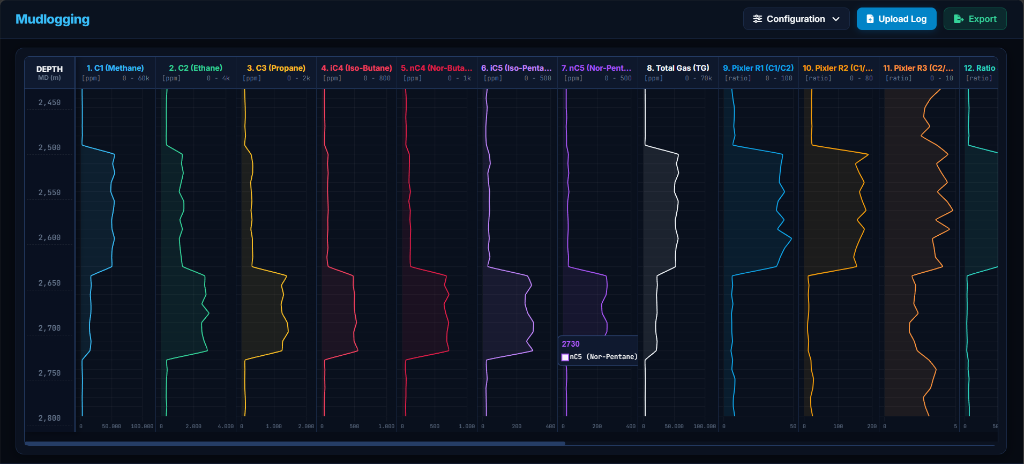
\includegraphics[width=\textwidth]{mockup_main_tracks.png}
    \caption{Main Application Interface featuring the 21-track continuous well log visualization with pinned left-hand Measured Depth ($MD$) axis and synchronous crosshair cursor.}
    \label{fig:mockup_main}
\end{figure}

\begin{figure}[H]
    \centering
    \begin{minipage}[t]{0.48\textwidth}
        \centering
        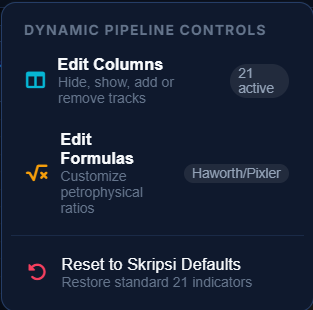
\includegraphics[width=\textwidth]{mockup_config_dropdown.png}
        \caption{Pipeline Controls dropdown menu in the top navigation bar.}
        \label{fig:mockup_config}
    \end{minipage}
    \hfill
    \begin{minipage}[t]{0.48\textwidth}
        \centering
        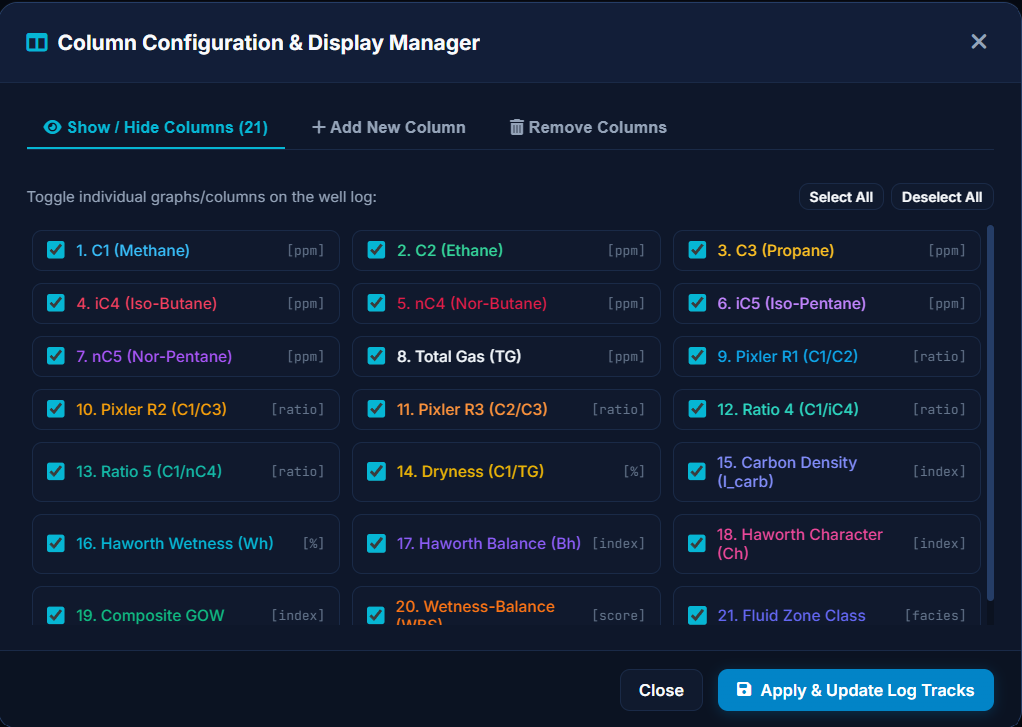
\includegraphics[width=\textwidth]{mockup_columns_manager.png}
        \caption{Column Configuration \& Display Manager modal for toggling and reordering tracks.}
        \label{fig:mockup_columns}
    \end{minipage}
\end{figure}

\begin{figure}[H]
    \centering
    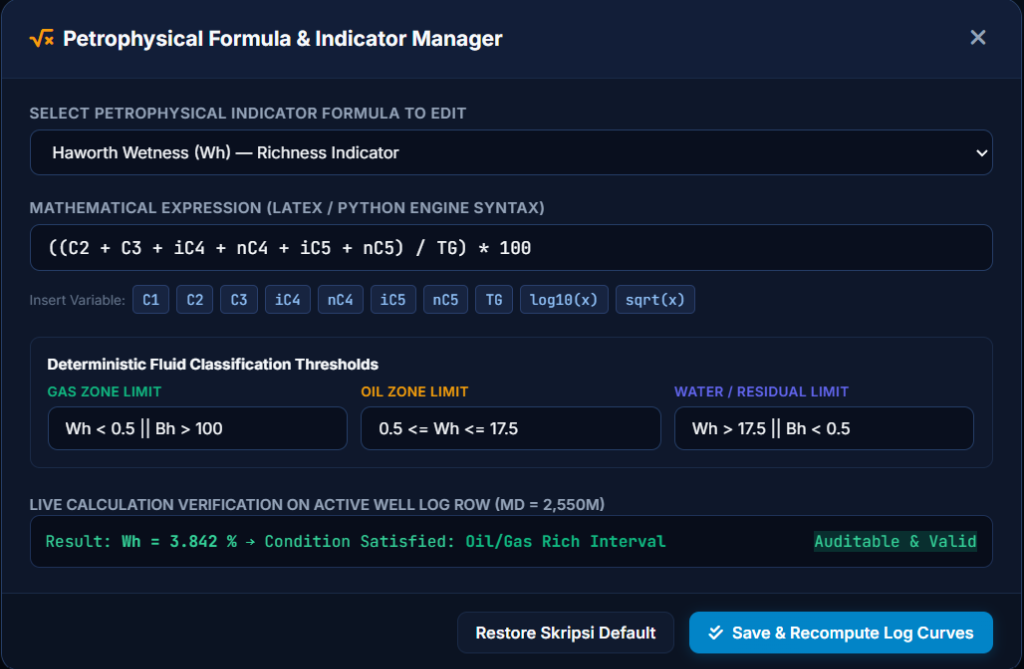
\includegraphics[width=0.88\textwidth]{mockup_formulas_manager.png}
    \caption{Petrophysical Formula \& Indicator Manager modal for live mathematical editing, variable insertion, threshold tuning, and real-time calculation preview.}
    \label{fig:mockup_formulas}
\end{figure}

\subsubsection{End-User Operational Workflow}

The application workflow is structured across four sequential stages designed to minimize operational friction:

\begin{enumerate}
    \item \textbf{Data Ingestion:} 
    The user uploads a mud logging or well logging file (\texttt{.csv}, \texttt{.txt}, \texttt{.xlsx}, or \texttt{.las}) through the file uploader. The ingestion pipeline extracts gas channels ($C_1 - C_5, TG$), normalizes depth measurements, calculates the 16 derived petrophysical indicators, executes fluid classification, and renders the 21-track visualization in under 5 seconds.

    \item \textbf{Well Log Exploration:} 
    Users analyze continuous depth trajectories with synchronized multi-track scrolling locked to the Measured Depth ($MD$) axis, inspecting numerical values via hover crosshairs and reviewing color-coded fluid zone classification overlays.

    \item \textbf{Track Display Customization (Edit Columns):} 
    Accessing the \textit{Column Configuration \& Display Manager} (Figure~\ref{fig:mockup_columns}) enables users to toggle the visibility of individual parameter tracks, adjust column sequences, and manage dataset schemas with immediate live updates.

    \item \textbf{Formula and Threshold Calibration (Edit Formulas):} 
    Through the \textit{Petrophysical Formula \& Indicator Manager} (Figure~\ref{fig:mockup_formulas}), users can modify indicator mathematical expressions using quick-insert variable tokens (e.g., $C_1 \dots C_5, TG, W_h, B_h, \log_{10}$), adjust classification cutoffs, and preview calculations live against active well log records.
\end{enumerate}

\section{Software Implementation}

The implementation translates the architectural design into modular, clean, and maintainable Python packages adhering to scientific software standards.

\subsection{Module Responsibilities}
The codebase is structured into four primary modules:
\begin{itemize}
    \item \texttt{parser.py}: Implements file decoding, format detection, header stripping, and missing-value normalization.
    \item \texttt{engine.py}: Encapsulates the declarative parameter graph, vectorized petrophysical formula pipelines, and deterministic fluid classification routines.
    \item \texttt{evaluator.py}: Houses ground-truth validation routines, confusion matrix calculation, and statistical performance benchmarking.
    \item \texttt{app.py}: Configures Dash application callbacks, binds user interactions, and renders responsive multi-track visual components.
\end{itemize}

\subsection{Deterministic Implementation Principles}
Because the calculation engine is purely deterministic—operating strictly on closed-form petrophysical formulas and explicit boundary thresholds—the system development requires no empirical training data or stochastic model fitting during construction. Algorithms are validated directly against analytical test matrices to guarantee mathematical fidelity.

\subsection{In-Memory Reactive State Execution}
The application executes entirely in memory. Uploaded well data is parsed, processed through vectorized NumPy and Pandas routines, and rendered across synchronized Plotly subplots, ensuring rapid execution without persistent server-side caching.

\section{System Verification and Performance Evaluation}

Validation follows a structured evaluation strategy covering four core dimensions: mathematical correctness, empirical classification accuracy, computational latency, and user experience.

\subsection{Algorithmic Unit Verification}
Algorithmic verification confirms that all coded formulas match their analytical mathematical definitions. Unit tests run against synthetic benchmark tensors with predefined inputs and outputs, ensuring zero floating-point drift or calculation errors across all 16 ratio indicators.

\subsection{Empirical Classification Accuracy and Ground-Truth Validation}
To evaluate the predictive correctness of the deterministic fluid classification engine, model predictions are benchmarked against ground-truth reservoir fluid contacts established by Wireline Formation Testers (RFT/MDT) and production well tests. The multi-class classification problem is evaluated across three primary reservoir fluid regimes:
\begin{equation}
    C = \{\text{Gas Zone}, \text{Oil Zone}, \text{Water / Non-Productive Sand}\}
\end{equation}

For each class $c \in C$, depth intervals are categorized in a confusion matrix as True Positives ($TP_c$), False Positives ($FP_c$), True Negatives ($TN_c$), and False Negatives ($FN_c$). Performance is quantified using standard classification metrics \citep{sokolova2009, powers2011}:

\begin{enumerate}
    \item \textbf{Overall Classification Accuracy:} Measures the total proportion of depth intervals correctly classified across all categories:
    \begin{equation}
        \text{Accuracy} = \frac{\sum_{c \in C} TP_c}{\sum_{c \in C} (TP_c + FP_c + FN_c)}
    \end{equation}

    \item \textbf{Precision (Positive Predictive Value):} Quantifies the proportion of predicted class $c$ intervals that are true reservoir pay zones:
    \begin{equation}
        \text{Precision}_c = \frac{TP_c}{TP_c + FP_c}
    \end{equation}

    \item \textbf{Recall (Sensitivity / True Positive Rate):} Measures the proportion of actual occurrences of fluid class $c$ correctly identified by the system:
    \begin{equation}
        \text{Recall}_c = \frac{TP_c}{TP_c + FN_c}
    \end{equation}

    \item \textbf{Class F1-Score:} The harmonic mean of Precision and Recall for class $c$:
    \begin{equation}
        F_{1, c} = 2 \times \frac{\text{Precision}_c \times \text{Recall}_c}{\text{Precision}_c + \text{Recall}_c}
    \end{equation}

    \item \textbf{Macro-Averaged F1-Score ($\text{Macro-}F_1$):} Provides an unweighted mean of F1-Scores across all classes, ensuring that minority classes (e.g., thin oil-bearing pay intervals) are evaluated with equal importance relative to dominant non-productive intervals \citep{sokolova2009}:
    \begin{equation}
        \text{Macro-}F_1 = \frac{1}{|C|} \sum_{c \in C} F_{1, c}
    \end{equation}
\end{enumerate}

\subsection{Computational Throughput Benchmarking ($\Delta t_{\text{total}} \le 5.0\text{ s}$)}
To evaluate operational speed in active wellsite environments, system efficiency is measured across the complete end-to-end processing pipeline:
\begin{equation}
    \Delta t_{\text{total}} = t_{\text{ingest}} + t_{\text{compute}} + t_{\text{render}}
\end{equation}
The target benchmark requires $\Delta t_{\text{total}} \le 5.0\text{ seconds}$ when processing dense mud logging datasets spanning full well trajectories ($> 3000\text{ m}$).

\subsection{User Experience and Usability Evaluation}

To assess operational usability, navigation fluency, and interface clarity, evaluation combines observational analysis with standardized usability benchmarking:

\subsubsection{Task-Oriented Behavioral Observation}
Domain practitioners (petrophysicists, operations geologists, and wellsite engineers) are observed during structured interpretation sessions using direct observation, interaction telemetry, and concurrent \textit{Think-Aloud Protocols} across four core workflows:
\begin{enumerate}
    \item \textbf{Data Ingestion Workflow:} Uploading raw field mud logs and observing automated channel detection. Evaluators' time-to-first-render and initial navigation choices are tracked.
    \item \textbf{Multi-Track Interpretation Workflow:} Inspecting continuous vertical tracks, utilizing crosshair tooltips, and identifying predicted fluid contacts.
    \item \textbf{Column Management Workflow:} Accessing the *Column Configuration Manager* to isolate targeted ratio groups and customize display layouts.
    \item \textbf{Formula and Threshold Tuning Workflow:} Utilizing the *Petrophysical Formula Manager* to modify indicator equations or adjust classification cutoffs with live preview verification.
\end{enumerate}

\subsubsection{Standardized Usability Benchmarking}
Following the observation session, participants complete a standardized evaluation questionnaire consisting of 10 targeted usability items rated on a linear scale from 1 (poor) to 10 (excellent). An evaluator's total score ($S_{\text{user}}$) is calculated by summing their ratings across all 10 items:
\begin{equation}
    S_{\text{user}} = \sum_{i=1}^{10} q_i
\end{equation}
where $q_i \in [1, 10]$ represents the rating for item $i$. The overall usability performance is measured by the average score ($\overline{S}$) across all $N$ evaluators:
\begin{equation}
    \overline{S} = \frac{1}{N} \sum_{k=1}^{N} S_{\text{user}, k}
\end{equation}
The benchmark target for the system is established at a mean total usability score of $\overline{S} > 68.0$ out of 100.

\section{Software Release and Deployment}

The final SDLC phase encompasses dependency management, software packaging, and open-source distribution.

\subsection{Packaging and Dependency Management}
Software dependencies are specified in a version-pinned \texttt{requirements.txt} manifest covering core libraries (\texttt{dash}, \texttt{dash-bootstrap-components}, \texttt{plotly}, \texttt{pandas}, \texttt{numpy}, and \texttt{openpyxl}), ensuring cross-platform reproducibility across Windows, Linux, and macOS environments.

\subsection{Open-Source Distribution and Accessibility}
The software is published under an open-source license on a public GitHub repository. The repository includes full source code, installation guides, dataset templates, and documentation to support transparent community verification and academic research in formation evaluation.